% Path-clustering algorithm walkthrough — all 7 steps in one vertical figure.
%
% Compile from this directory:
%   pdflatex steps_overview.tex
%
% Or include in a paper as a full-width figure:
%   \begin{figure*}[t]
%     \centering
%     \includegraphics[width=\textwidth]{figures/path_clustering_walkthrough/steps_overview.pdf}
%     \caption{…}
%   \end{figure*}
%
% Colour palette matches the companion TikZ diagram (Wong 2011 colorblind-safe):
%   cbBlue   #0072B2   cbOrange  #D55E00   cbGrey   #999999
%   charcoal #2E2E2E   boxBg    #F8F9F9

\documentclass[border=6pt]{standalone}
\usepackage{graphicx}
\usepackage{xcolor}
\usepackage{tikz}
\usetikzlibrary{positioning, backgrounds, fit}

% ── palette ─────────────────────────────────────────────────────────────────
\definecolor{cbBlue}{HTML}{0072B2}
\definecolor{cbOrange}{HTML}{D55E00}
\definecolor{cbGrey}{HTML}{999999}
\definecolor{charcoal}{HTML}{2E2E2E}
\definecolor{boxBg}{HTML}{F8F9F9}

\begin{document}
\sffamily

\begin{tikzpicture}[
  % panel box around each figure
  panel/.style={
    inner sep=3pt,
    draw=cbBlue!35,
    fill=boxBg,
    rounded corners=4pt,
    line width=0.7pt,
  },
  % circular step-number badge (top-left of each panel)
  badge/.style={
    circle,
    fill=cbBlue,
    text=white,
    font=\footnotesize\bfseries\sffamily,
    inner sep=1.5pt,
    minimum size=14pt,
    anchor=north west,
  },
  % caption label to the right of each panel
  subcap/.style={
    font=\scriptsize\sffamily,
    text=charcoal,
    align=left,
    text width=3.6cm,
  },
  % arrow between panels
  stepArrow/.style={
    ->,
    charcoal!60,
    line width=1pt,
    shorten >=2pt,
    shorten <=2pt,
  },
]

% ── figure width (all panels share this width) ─────────────────────────────
\newlength{\FW}
\setlength{\FW}{14cm}

% ── step 1: cluster extraction ──────────────────────────────────────────────
\node[panel] (s1)
  {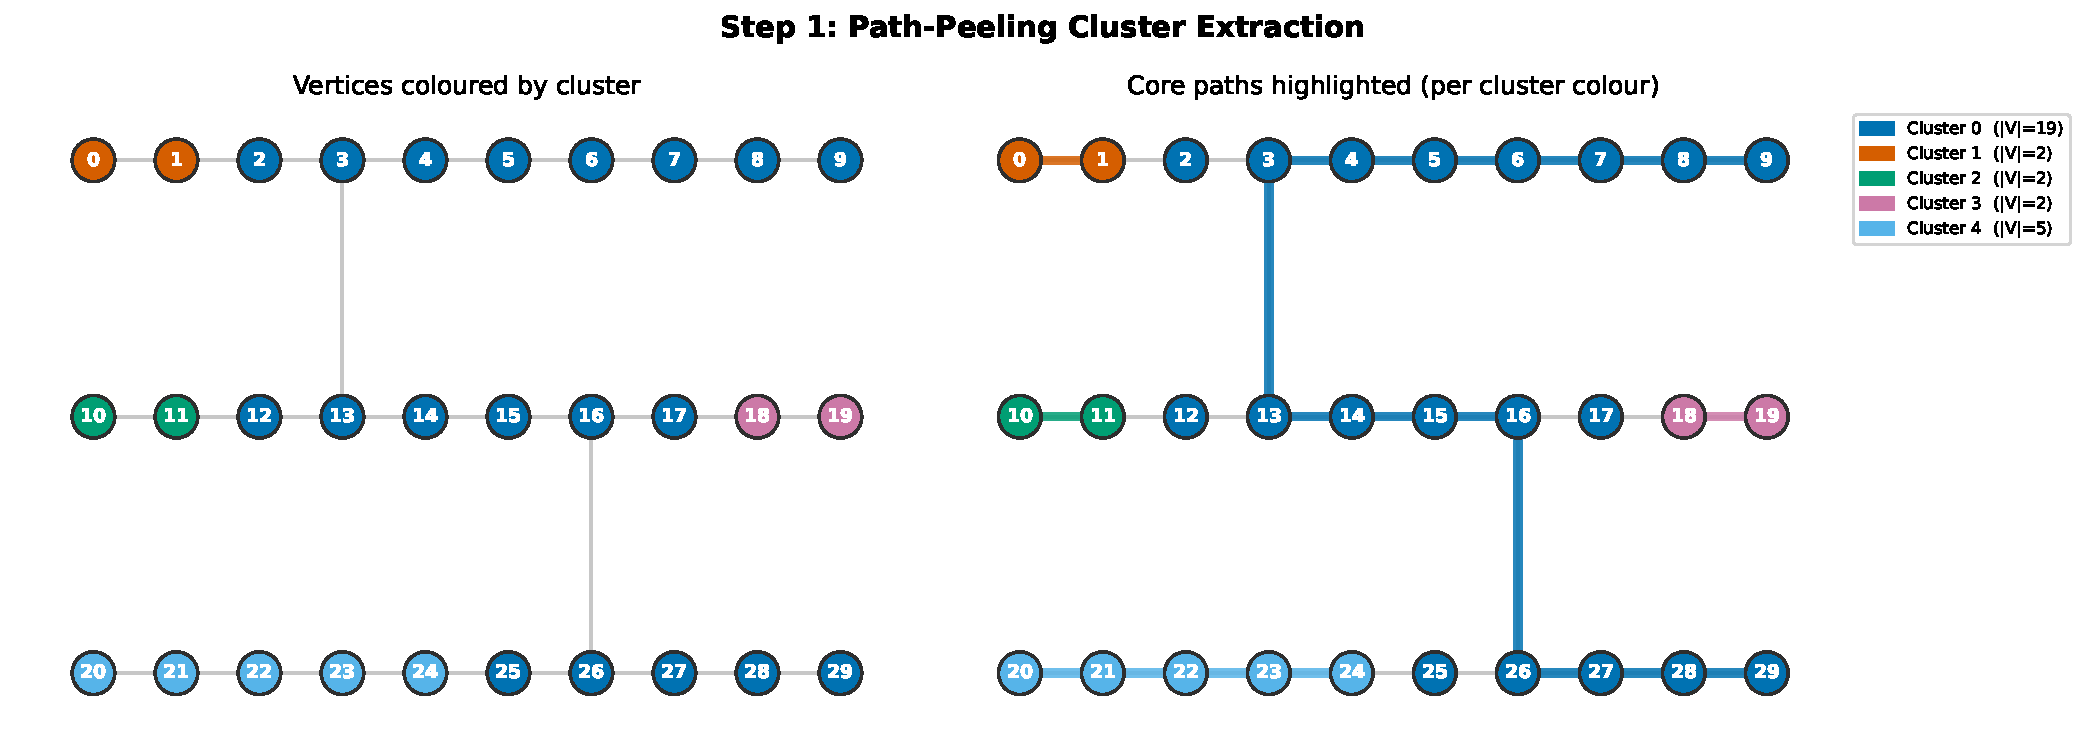
\includegraphics[width=\FW]{01_cluster_extraction.pdf}};
\node[badge] at (s1.north west) {1};
\node[subcap, right=4mm of s1.north east, anchor=north west] (c1)
  {\textcolor{cbBlue}{\textbf{Step 1}}\\Path-peeling\\cluster extraction};

% ── step 2: cluster meta-graph ──────────────────────────────────────────────
\node[panel, below=4mm of s1] (s2)
  {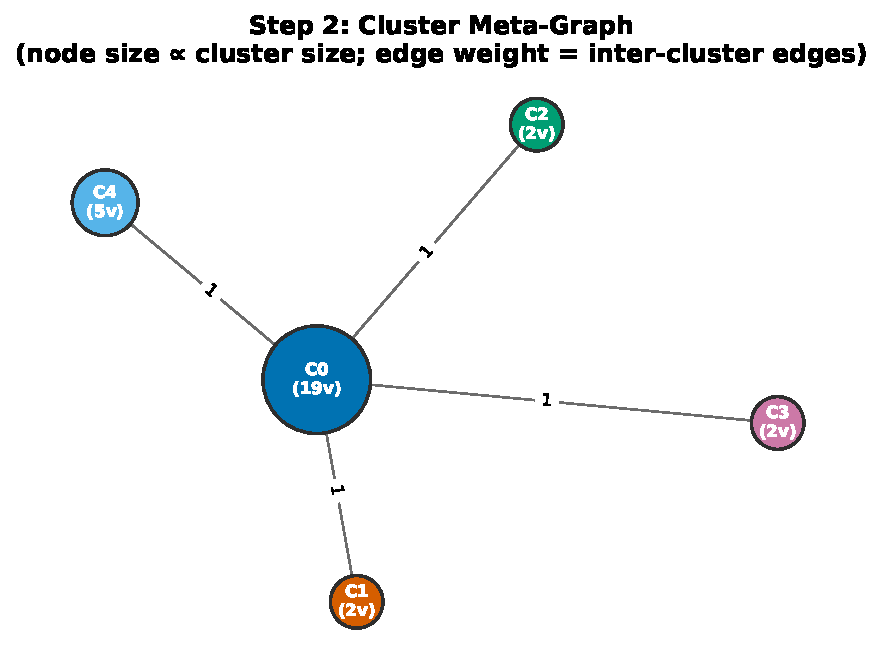
\includegraphics[width=\FW]{02_cluster_metagraph.pdf}};
\node[badge] at (s2.north west) {2};
\node[subcap, right=4mm of s2.north east, anchor=north west] (c2)
  {\textcolor{cbBlue}{\textbf{Step 2}}\\Cluster\\meta-graph};

% ── step 3: inter-cluster ordering ──────────────────────────────────────────
\node[panel, below=4mm of s2] (s3)
  {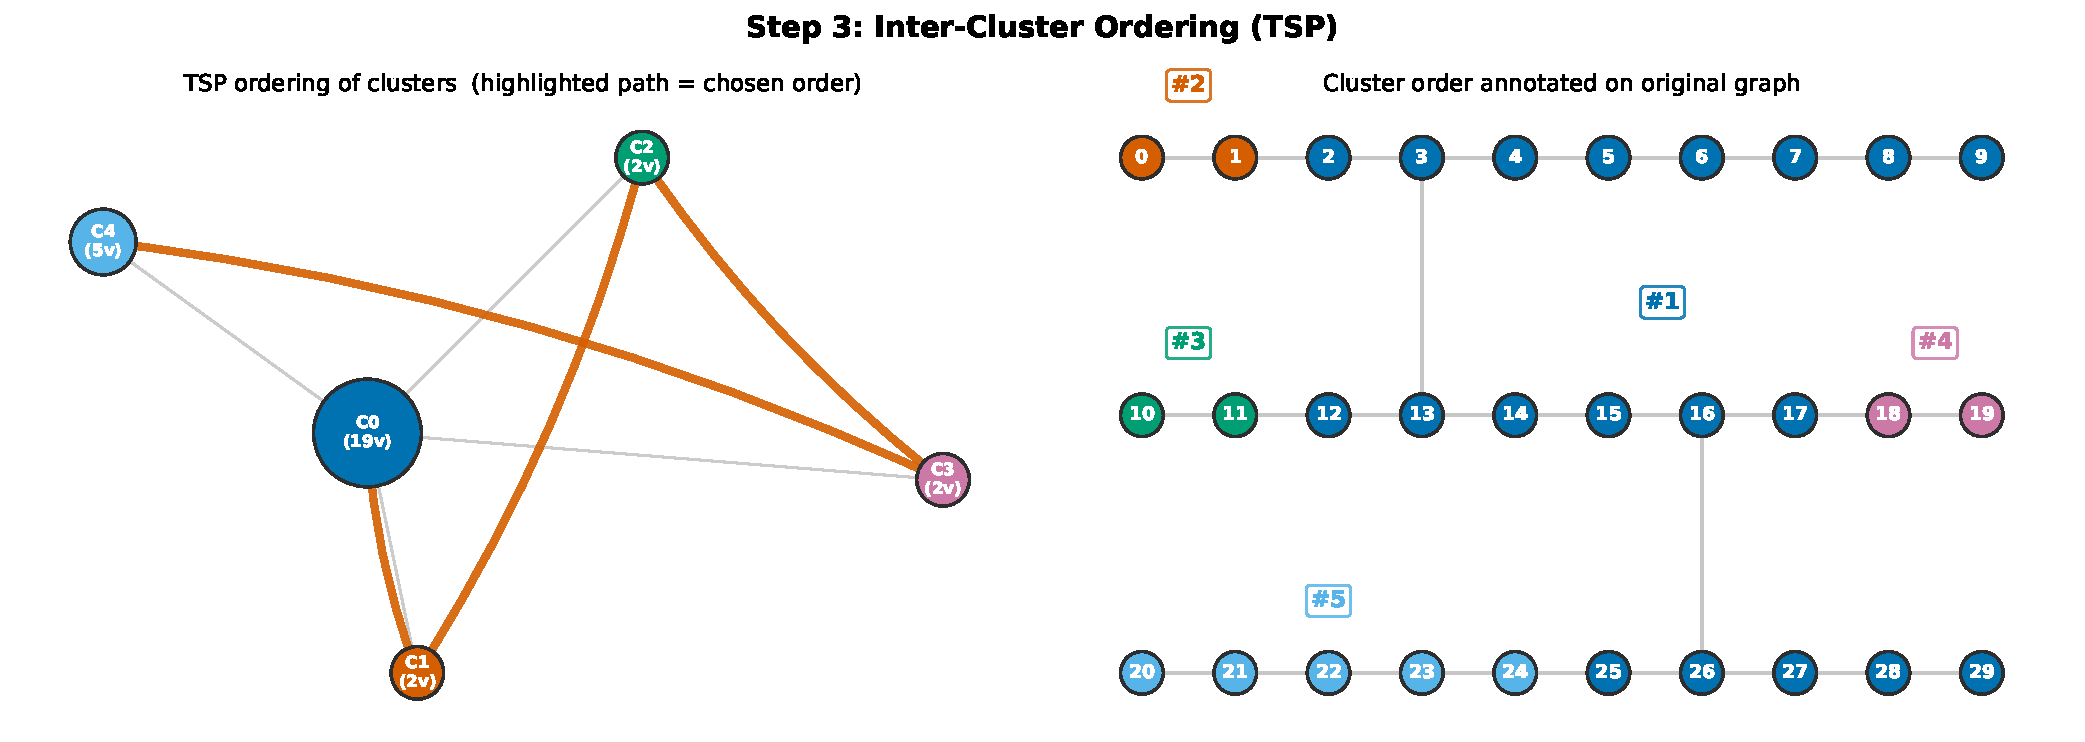
\includegraphics[width=\FW]{03_cluster_ordering.pdf}};
\node[badge] at (s3.north west) {3};
\node[subcap, right=4mm of s3.north east, anchor=north west] (c3)
  {\textcolor{cbBlue}{\textbf{Step 3}}\\Inter-cluster\\ordering (TSP)};

% ── step 4: intra-cluster ordering ──────────────────────────────────────────
\node[panel, below=4mm of s3] (s4)
  {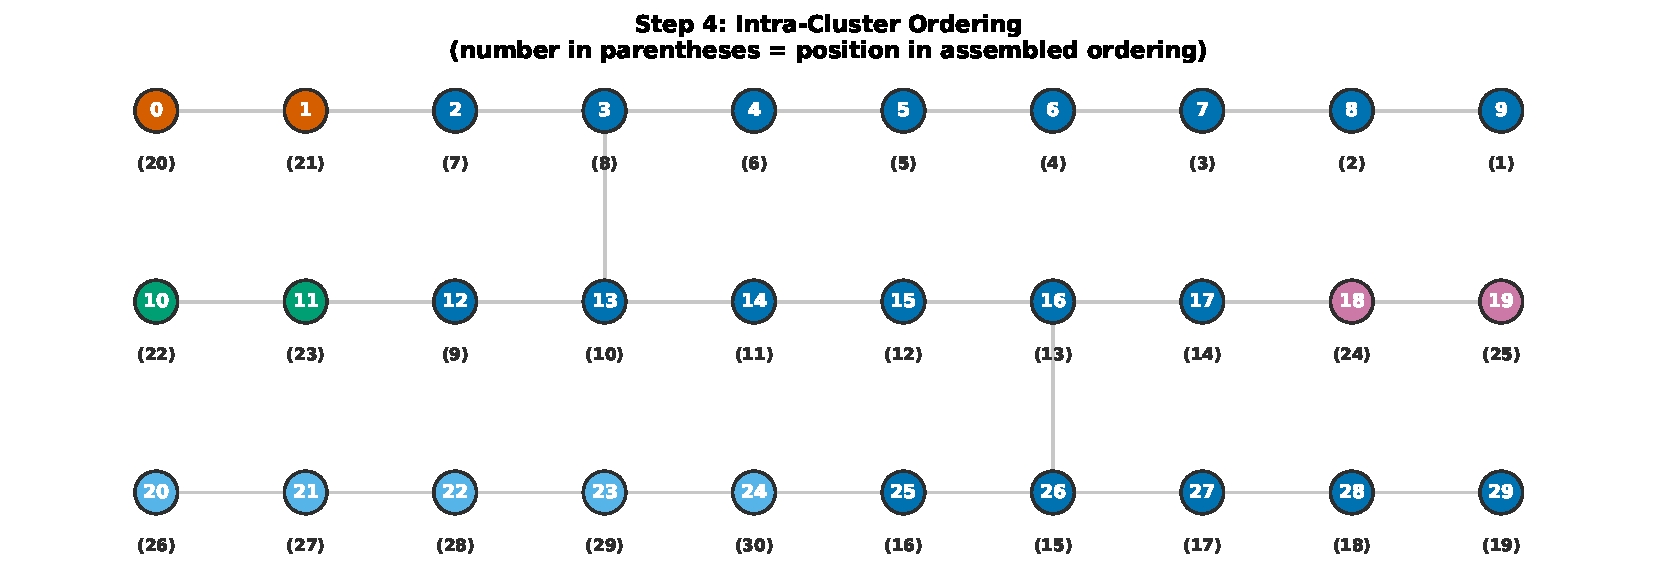
\includegraphics[width=\FW]{04_intra_cluster_ordering.pdf}};
\node[badge] at (s4.north west) {4};
\node[subcap, right=4mm of s4.north east, anchor=north west] (c4)
  {\textcolor{cbBlue}{\textbf{Step 4}}\\Intra-cluster\\ordering};

% ── step 5: assembled ordering + height function ─────────────────────────────
\node[panel, below=4mm of s4] (s5)
  {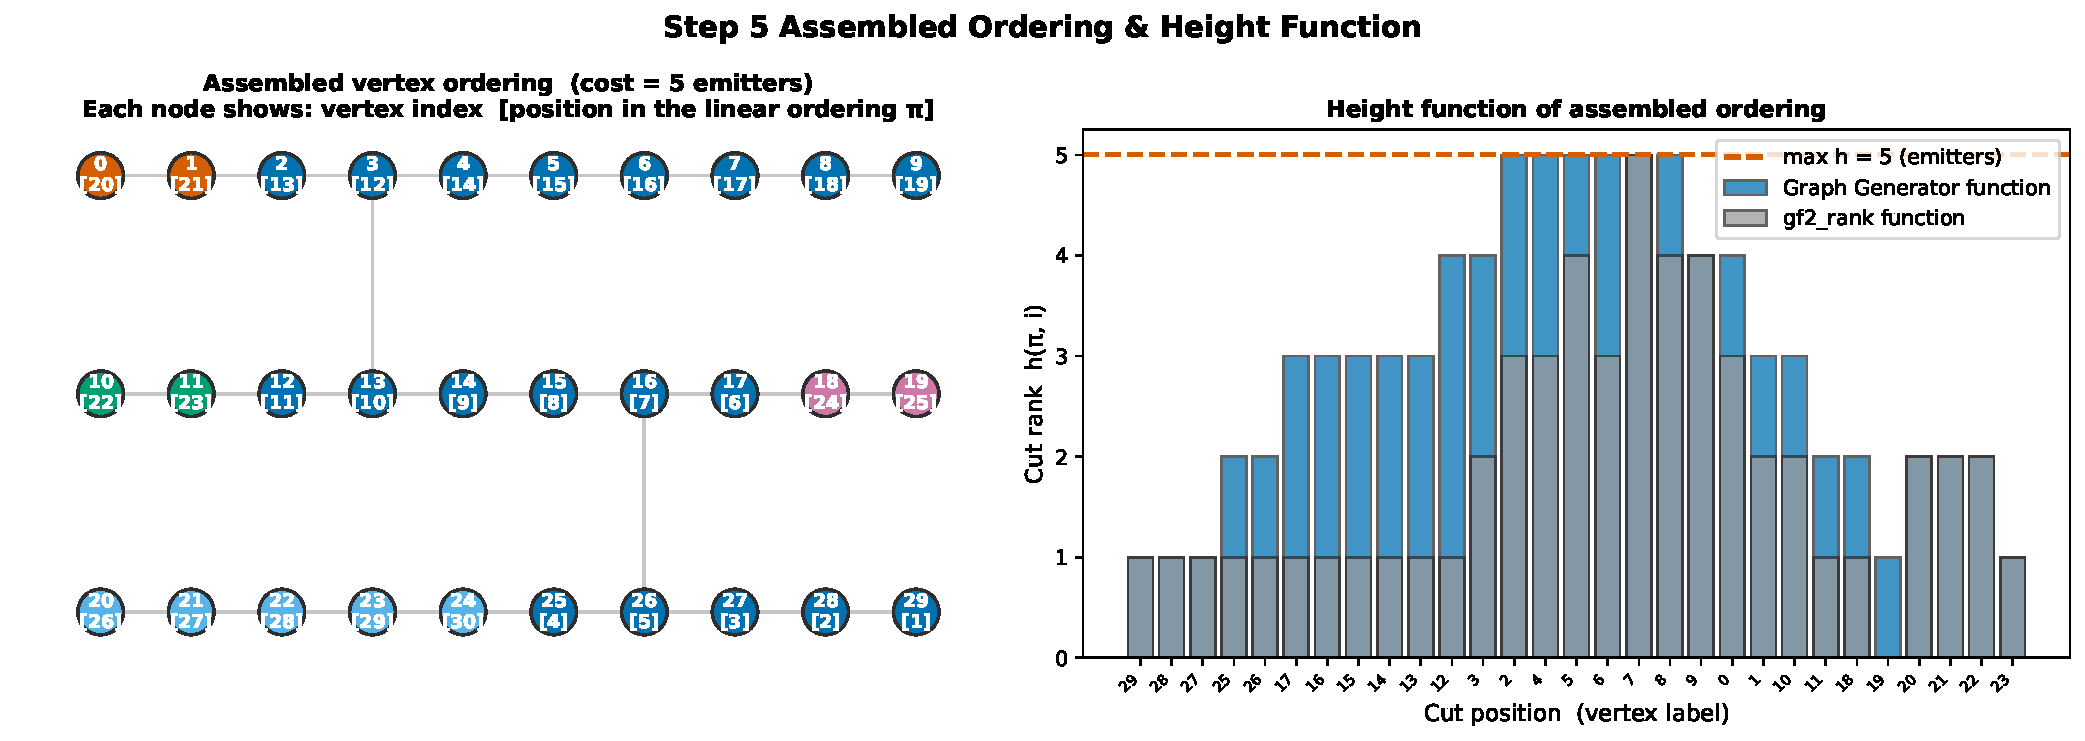
\includegraphics[width=\FW]{05_assembled_ordering_height.pdf}};
\node[badge] at (s5.north west) {5};
\node[subcap, right=4mm of s5.north east, anchor=north west] (c5)
  {\textcolor{cbBlue}{\textbf{Step 5}}\\Assembled ordering\\+ height function};

% ── step 6: boundary vertices ────────────────────────────────────────────────
\node[panel, below=4mm of s5] (s6)
  {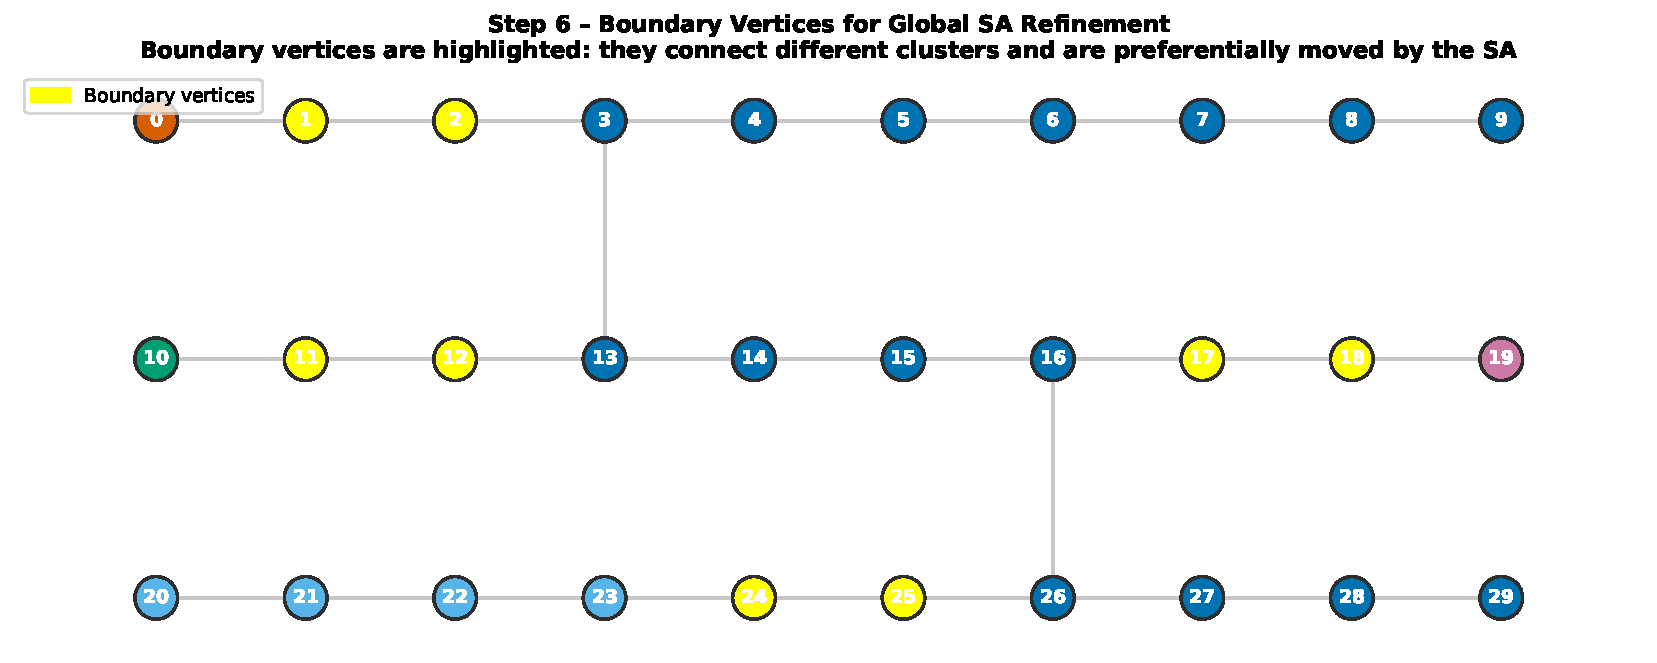
\includegraphics[width=\FW]{06_boundary_vertices.pdf}};
\node[badge] at (s6.north west) {6};
\node[subcap, right=4mm of s6.north east, anchor=north west] (c6)
  {\textcolor{cbBlue}{\textbf{Step 6}}\\Boundary vertices\\for SA refinement};

% ── step 7: global SA refinement ────────────────────────────────────────────
\node[panel, below=4mm of s6] (s7)
  {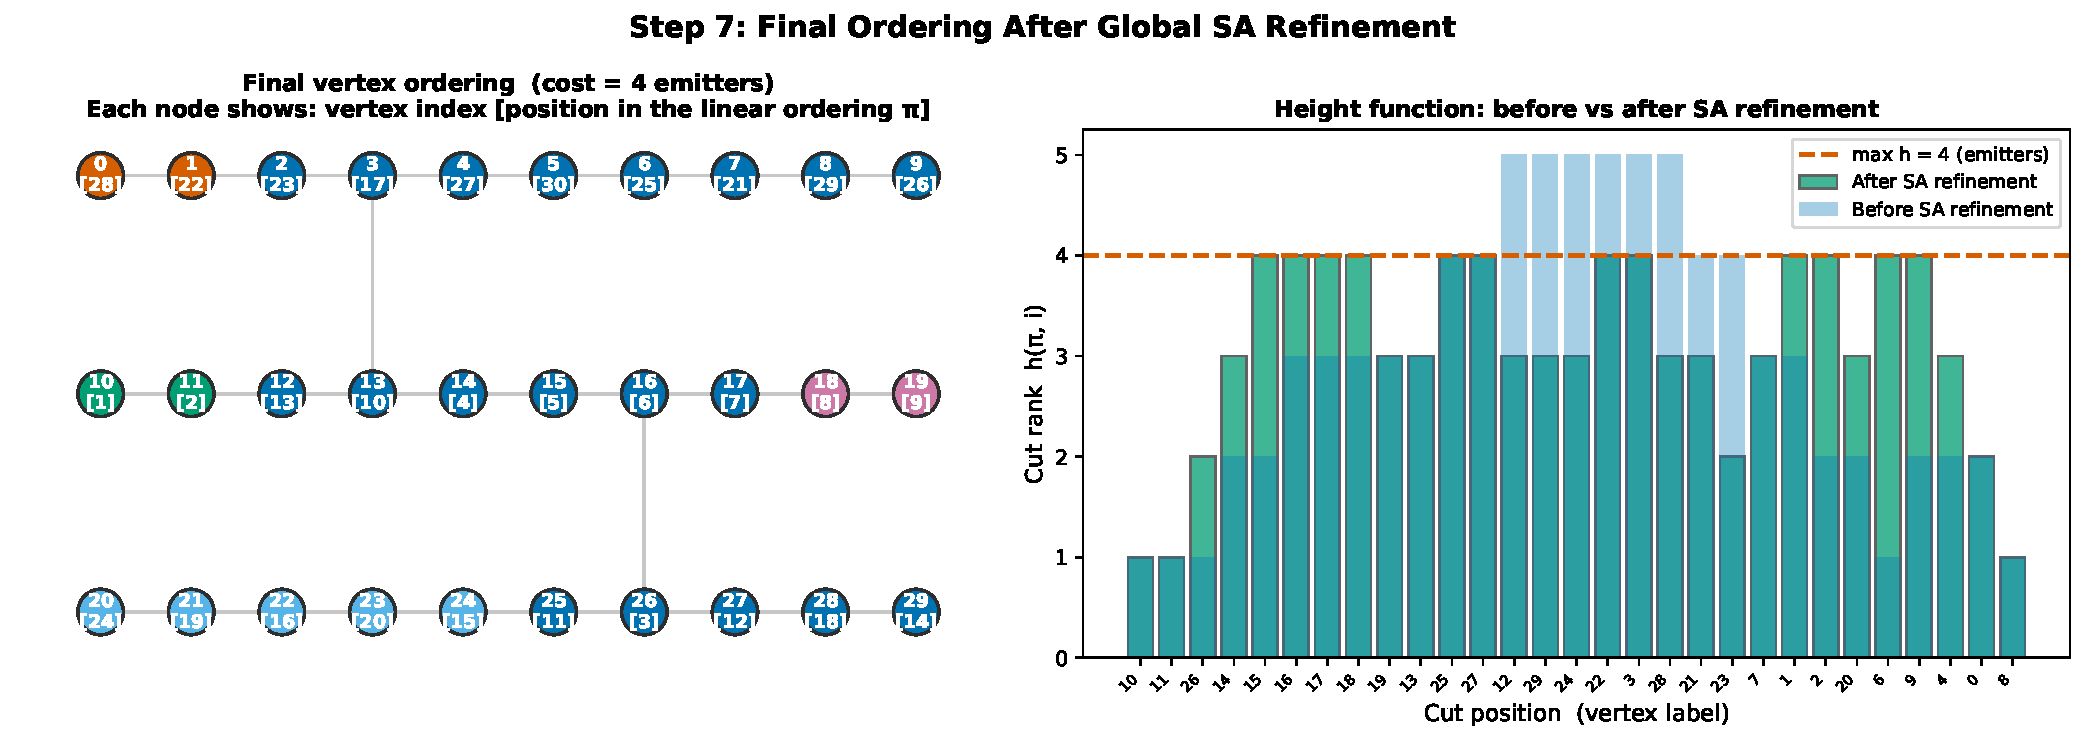
\includegraphics[width=\FW]{07_final_ordering_sa_refinement.pdf}};
\node[badge] at (s7.north west) {7};
\node[subcap, right=4mm of s7.north east, anchor=north west] (c7)
  {\textcolor{cbBlue}{\textbf{Step 7}}\\Global SA\\refinement};

% ── arrows ───────────────────────────────────────────────────────────────────
\foreach \a/\b in {s1/s2, s2/s3, s3/s4, s4/s5, s5/s6, s6/s7}{
  \draw[stepArrow] (\a.south) -- (\b.north);
}

% ── orange result badge to the right of step 7 ──────────────────────────────
\node[
  draw=cbOrange, fill=cbOrange!8, rounded corners=3pt,
  line width=0.8pt,
  font=\scriptsize\bfseries\sffamily,
  text=cbOrange,
  inner sep=3pt,
  below=4mm of s7.south,
  anchor=north,
] {Final result: $\widehat{lrw}$\,=\,4 emitters};

\end{tikzpicture}
\end{document}
